\documentclass[10pt,a4paper]{article}
\usepackage[utf8]{inputenc}
\usepackage[francais]{babel}
\usepackage[T1]{fontenc}
\usepackage{amsmath}
\usepackage{amsfonts}
\usepackage{amssymb}
\usepackage{graphicx}
\usepackage{enumitem}
\usepackage{lmodern}
\usepackage{listings}
\usepackage{color}
\usepackage{tikz}

\definecolor{mygreen}{rgb}{0,0.6,0}
\definecolor{mygray}{rgb}{0.5,0.5,0.5}
\definecolor{mymauve}{rgb}{0.58,0,0.82}

\lstset{ %
  backgroundcolor=\color{white},   % choose the background color; you must add \usepackage{color} or \usepackage{xcolor}
  basicstyle=\footnotesize,        % the size of the fonts that are used for the code
  breakatwhitespace=false,         % sets if automatic breaks should only happen at whitespace
  breaklines=true,                 % sets automatic line breaking
  captionpos=b,                    % sets the caption-position to bottom
  commentstyle=\color{mygreen},    % comment style
  deletekeywords={...},            % if you want to delete keywords from the given language
  escapeinside={\%*}{*)},          % if you want to add LaTeX within your code
  extendedchars=true,              % lets you use non-ASCII characters; for 8-bits encodings only, does not work with UTF-8
  frame=single,                    % adds a frame around the code
  keepspaces=true,                 % keeps spaces in text, useful for keeping indentation of code (possibly needs columns=flexible)
  keywordstyle=\color{blue},       % keyword style
  language=Java,                   % the language of the code
  morekeywords={*,...},            % if you want to add more keywords to the set
  numbers=left,                    % where to put the line-numbers; possible values are (none, left, right)
  numbersep=5pt,                   % how far the line-numbers are from the code
  numberstyle=\tiny\color{mygray}, % the style that is used for the line-numbers
  rulecolor=\color{black},         % if not set, the frame-color may be changed on line-breaks within not-black text (e.g. comments (green here))
  showspaces=false,                % show spaces everywhere adding particular underscores; it overrides 'showstringspaces'
  showstringspaces=false,          % underline spaces within strings only
  showtabs=false,                  % show tabs within strings adding particular underscores
  stepnumber=2,                    % the step between two line-numbers. If it's 1, each line will be numbered
  stringstyle=\color{mymauve},     % string literal style
  tabsize=4,                       % sets default tabsize to 2 spaces
  title=\lstname                   % show the filename of files included with \lstinputlisting; also try caption instead of title
}
\usepackage[left=2cm,right=2cm,top=2cm,bottom=2cm]{geometry}


\date{Vendredi 14 Novembre 2014}
\author{Groupe 2.2}
\title{Mission 4 : Rapport Final}
\begin{document}
\maketitle
\section*{Introduction}

Il était demandé d'élargir l'implémentation de notre mission 3 afin d'ajouter de nouvelles fonctionnalités comme lister toutes les revues d’un domaine donné,  par ordre alphabétique, lister toutes les revues d’un domaine par rang du classement et, pour un rang donné, par ordre alphabétique, . . .

\section*{Choix d'implémentation}

Nous avons trois grandes types de recherche possibles : la recherche d'une seule publication, la recherche de l'ensemble des publications présentes et les recherches multicritères. 

\subsection*{Recherche d'une seule publication}

Nous avons repris l'implémentation de la mission 3.  Celle-ci permet de retrouver une publication dans une hashMap. Pour plus d'information sur le fonctionnement de la hashMap, nous vous invitons à relire le rapport de la mission 3.

\subsection*{Recherche de l'ensemble des publications} 

Nous avons pris la décision de favoriser la complexité temporelle par rapport à la complexité spatiale. Nous avons donc créé une arrayList triée par ordre alphabétique afin de retourner d'une seule fois l'ensemble des publications.

\subsection*{Recherches multicritères}

Nous avons scindé l'ensemble des publications en sous-ensemble selon leur rang. Dans notre cas, nous avons donc 5 sous-ensembles ($A*$,A,B,C,D). La recherche dans un des sous-ensembles sera plus efficace que dans l'ensemble complet par le simple fait qu'il y a moins d'élément. Les sous-ensembles sont représentés par des TreeMap qui contiennent comme clé des noms de domaines et comme valeur des listes de référence de publication lié au nom de domaine. L'utilisation de référence n'augmente pas significativement notre complexité spatiale.

\section*{Diagramme de classe}
\begin{center}
    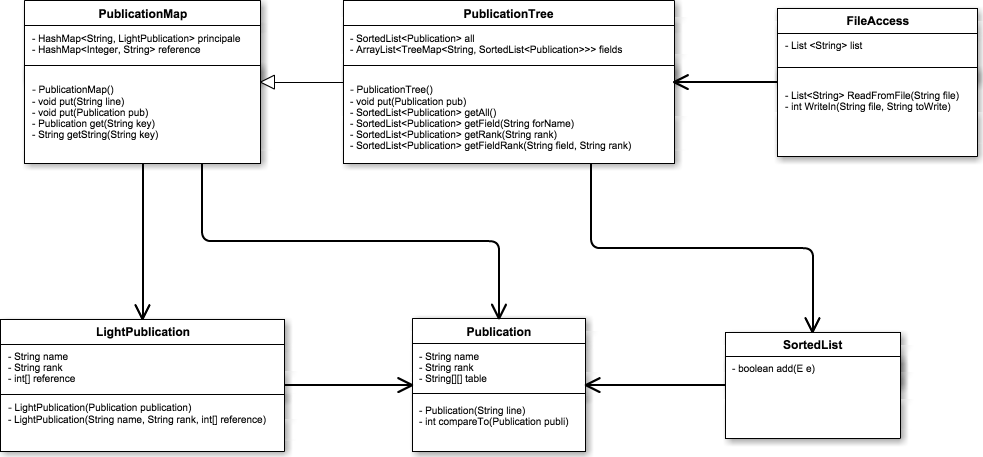
\includegraphics[scale=0.5]{UML.png}
\end{center}

\section*{Conclusion}
La décomposition des classes dans notre programme, nous a facilité la répartition des taches, l'utilisation de multiple classe permet aussi de pouvoir être plus modulable. Tant au niveau de la repartition du travail, qu'au niveau de l'ajout de nouvelles fonctions pour adapter notre programme.\\
Nous avons essentiellement accès notre travail sur la minimisation du temps mis pour une recherche quelconque et nous avons donc fait moins attention à l'espace utilisé par le fonctionnement de notre programme.
Malgré le fait que nous ayons conçu notre programme à partir d'un exemple spécifique, la gestion d'une bibliothèque de revues scientifiques, nous pourrions élargir le modèle de notre programme pour la gestion d'une bibliothèque ou d'une médiathèque en créant des nouvelles classes héritant de la classe Publication.

\end{document}